\documentclass[twoside]{book}

% Packages required by doxygen
\usepackage{calc}
\usepackage{doxygen}
\usepackage{graphicx}
\usepackage[utf8]{inputenc}
\usepackage{makeidx}
\usepackage{multicol}
\usepackage{multirow}
\usepackage{textcomp}
\usepackage[table]{xcolor}

% Font selection
\usepackage[T1]{fontenc}
\usepackage{mathptmx}
\usepackage[scaled=.90]{helvet}
\usepackage{courier}
\usepackage{amssymb}
\usepackage{sectsty}
\renewcommand{\familydefault}{\sfdefault}
\allsectionsfont{%
  \fontseries{bc}\selectfont%
  \color{darkgray}%
}
\renewcommand{\DoxyLabelFont}{%
  \fontseries{bc}\selectfont%
  \color{darkgray}%
}

% Page & text layout
\usepackage{geometry}
\geometry{%
  a4paper,%
  top=2.5cm,%
  bottom=2.5cm,%
  left=2.5cm,%
  right=2.5cm%
}
\tolerance=750
\hfuzz=15pt
\hbadness=750
\setlength{\emergencystretch}{15pt}
\setlength{\parindent}{0cm}
\setlength{\parskip}{0.2cm}
\makeatletter
\renewcommand{\paragraph}{%
  \@startsection{paragraph}{4}{0ex}{-1.0ex}{1.0ex}{%
    \normalfont\normalsize\bfseries\SS@parafont%
  }%
}
\renewcommand{\subparagraph}{%
  \@startsection{subparagraph}{5}{0ex}{-1.0ex}{1.0ex}{%
    \normalfont\normalsize\bfseries\SS@subparafont%
  }%
}
\makeatother

% Headers & footers
\usepackage{fancyhdr}
\pagestyle{fancyplain}
\fancyhead[LE]{\fancyplain{}{\bfseries\thepage}}
\fancyhead[CE]{\fancyplain{}{}}
\fancyhead[RE]{\fancyplain{}{\bfseries\leftmark}}
\fancyhead[LO]{\fancyplain{}{\bfseries\rightmark}}
\fancyhead[CO]{\fancyplain{}{}}
\fancyhead[RO]{\fancyplain{}{\bfseries\thepage}}
\fancyfoot[LE]{\fancyplain{}{}}
\fancyfoot[CE]{\fancyplain{}{}}
\fancyfoot[RE]{\fancyplain{}{\bfseries\scriptsize Generated on Sun Apr 20 2014 20\-:13\-:11 for Noesis\-Leadwerks\-Wrapper by Doxygen }}
\fancyfoot[LO]{\fancyplain{}{\bfseries\scriptsize Generated on Sun Apr 20 2014 20\-:13\-:11 for Noesis\-Leadwerks\-Wrapper by Doxygen }}
\fancyfoot[CO]{\fancyplain{}{}}
\fancyfoot[RO]{\fancyplain{}{}}
\renewcommand{\footrulewidth}{0.4pt}
\renewcommand{\chaptermark}[1]{%
  \markboth{#1}{}%
}
\renewcommand{\sectionmark}[1]{%
  \markright{\thesection\ #1}%
}

% Indices & bibliography
\usepackage{natbib}
\usepackage[titles]{tocloft}
\setcounter{tocdepth}{3}
\setcounter{secnumdepth}{5}
\makeindex

% Hyperlinks (required, but should be loaded last)
\usepackage{ifpdf}
\ifpdf
  \usepackage[pdftex,pagebackref=true]{hyperref}
\else
  \usepackage[ps2pdf,pagebackref=true]{hyperref}
\fi
\hypersetup{%
  colorlinks=true,%
  linkcolor=blue,%
  citecolor=blue,%
  unicode%
}

% Custom commands
\newcommand{\clearemptydoublepage}{%
  \newpage{\pagestyle{empty}\cleardoublepage}%
}


%===== C O N T E N T S =====

\begin{document}

% Titlepage & ToC
\hypersetup{pageanchor=false}
\pagenumbering{roman}
\begin{titlepage}
\vspace*{7cm}
\begin{center}%
{\Large Noesis\-Leadwerks\-Wrapper \\[1ex]\large 0.\-41 }\\
\vspace*{1cm}
{\large Generated by Doxygen 1.8.6}\\
\vspace*{0.5cm}
{\small Sun Apr 20 2014 20:13:11}\\
\end{center}
\end{titlepage}
\clearemptydoublepage
\tableofcontents
\clearemptydoublepage
\pagenumbering{arabic}
\hypersetup{pageanchor=true}

%--- Begin generated contents ---
\chapter{Class Index}
\section{Class List}
Here are the classes, structs, unions and interfaces with brief descriptions\-:\begin{DoxyCompactList}
\item\contentsline{section}{\hyperlink{class_open_g_l_state}{Open\-G\-L\-State} \\*Stores and restores the current G\-P\-U state }{\pageref{class_open_g_l_state}}{}
\item\contentsline{section}{\hyperlink{struct_render_states}{Render\-States} }{\pageref{struct_render_states}}{}
\item\contentsline{section}{\hyperlink{class_u_i_renderer}{U\-I\-Renderer} \\*X\-A\-M\-L Renderer }{\pageref{class_u_i_renderer}}{}
\item\contentsline{section}{\hyperlink{class_u_i_render_target}{U\-I\-Render\-Target} \\*Render target }{\pageref{class_u_i_render_target}}{}
\item\contentsline{section}{\hyperlink{class_u_i_system}{U\-I\-System} \\*Manages all U\-I related renderers }{\pageref{class_u_i_system}}{}
\end{DoxyCompactList}

\chapter{Class Documentation}
\hypertarget{class_open_g_l_state}{\section{Open\-G\-L\-State Class Reference}
\label{class_open_g_l_state}\index{Open\-G\-L\-State@{Open\-G\-L\-State}}
}


Stores and restores the current G\-P\-U state.  




{\ttfamily \#include $<$Open\-G\-L\-State.\-h$>$}



Collaboration diagram for Open\-G\-L\-State\-:
\nopagebreak
\begin{figure}[H]
\begin{center}
\leavevmode
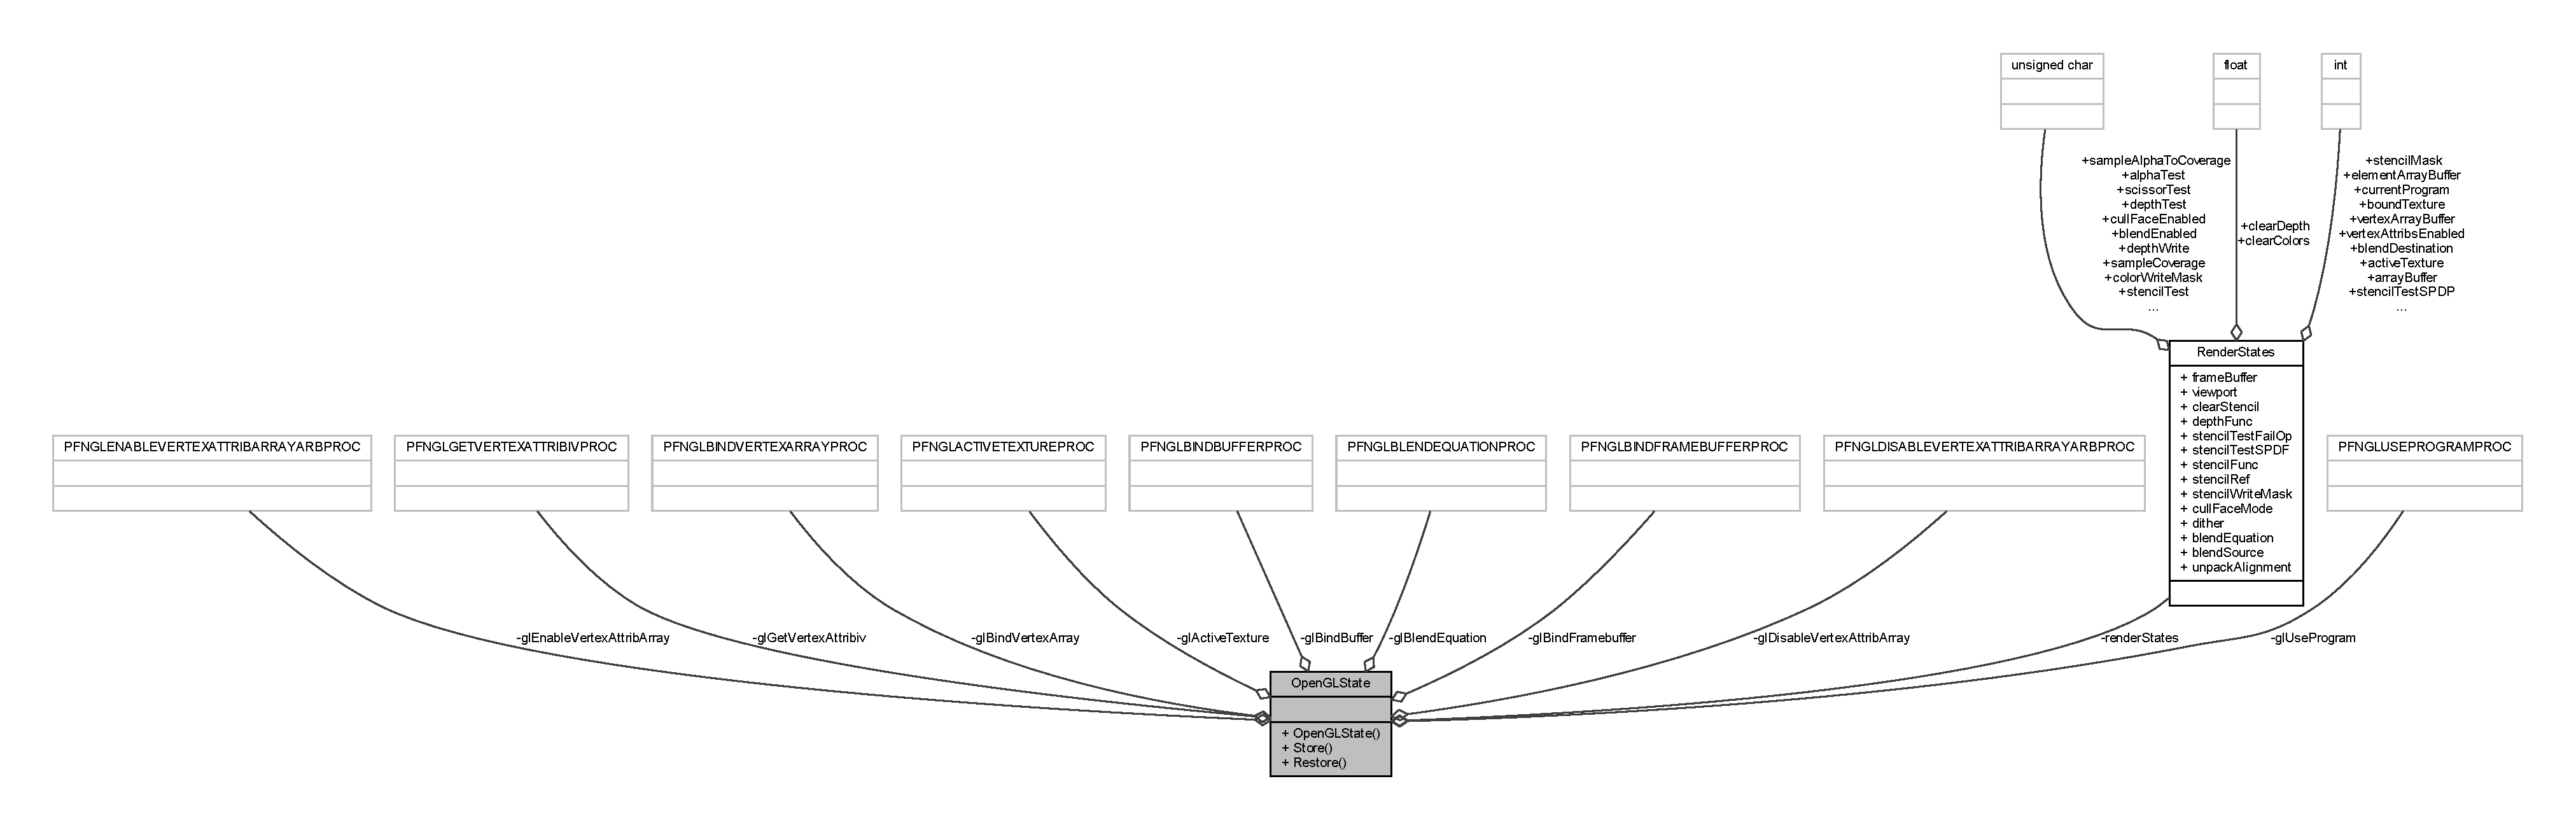
\includegraphics[width=350pt]{class_open_g_l_state__coll__graph}
\end{center}
\end{figure}
\subsection*{Public Member Functions}
\begin{DoxyCompactItemize}
\item 
\hypertarget{class_open_g_l_state_a8078b65f6b29b681960ba03b6d35160e}{void \hyperlink{class_open_g_l_state_a8078b65f6b29b681960ba03b6d35160e}{Store} ()}\label{class_open_g_l_state_a8078b65f6b29b681960ba03b6d35160e}

\begin{DoxyCompactList}\small\item\em Stores the current gpu state. \end{DoxyCompactList}\item 
\hypertarget{class_open_g_l_state_a08189bfef75f3408539b1e570d14d838}{void \hyperlink{class_open_g_l_state_a08189bfef75f3408539b1e570d14d838}{Restore} ()}\label{class_open_g_l_state_a08189bfef75f3408539b1e570d14d838}

\begin{DoxyCompactList}\small\item\em Restores the stored gpu state. \end{DoxyCompactList}\end{DoxyCompactItemize}
\subsection*{Private Attributes}
\begin{DoxyCompactItemize}
\item 
\hypertarget{class_open_g_l_state_a52e2325cc665c673b59eb43ce611a841}{\hyperlink{struct_render_states}{Render\-States} {\bfseries render\-States}}\label{class_open_g_l_state_a52e2325cc665c673b59eb43ce611a841}

\item 
\hypertarget{class_open_g_l_state_a580ee79f804a92e55b95c4910b2254e5}{P\-F\-N\-G\-L\-B\-I\-N\-D\-F\-R\-A\-M\-E\-B\-U\-F\-F\-E\-R\-P\-R\-O\-C {\bfseries gl\-Bind\-Framebuffer}}\label{class_open_g_l_state_a580ee79f804a92e55b95c4910b2254e5}

\item 
\hypertarget{class_open_g_l_state_a190e392c9aad9ccef7e947b7273c7522}{P\-F\-N\-G\-L\-B\-I\-N\-D\-B\-U\-F\-F\-E\-R\-P\-R\-O\-C {\bfseries gl\-Bind\-Buffer}}\label{class_open_g_l_state_a190e392c9aad9ccef7e947b7273c7522}

\item 
\hypertarget{class_open_g_l_state_a4522af78a19fa306ecae319663411014}{P\-F\-N\-G\-L\-A\-C\-T\-I\-V\-E\-T\-E\-X\-T\-U\-R\-E\-P\-R\-O\-C {\bfseries gl\-Active\-Texture}}\label{class_open_g_l_state_a4522af78a19fa306ecae319663411014}

\item 
\hypertarget{class_open_g_l_state_a9d20b98a10b8deff956ad4a788f2790e}{P\-F\-N\-G\-L\-U\-S\-E\-P\-R\-O\-G\-R\-A\-M\-P\-R\-O\-C {\bfseries gl\-Use\-Program}}\label{class_open_g_l_state_a9d20b98a10b8deff956ad4a788f2790e}

\item 
\hypertarget{class_open_g_l_state_a3a5d55d76a431489f0e038c31e14cfc1}{P\-F\-N\-G\-L\-G\-E\-T\-V\-E\-R\-T\-E\-X\-A\-T\-T\-R\-I\-B\-I\-V\-P\-R\-O\-C {\bfseries gl\-Get\-Vertex\-Attribiv}}\label{class_open_g_l_state_a3a5d55d76a431489f0e038c31e14cfc1}

\item 
\hypertarget{class_open_g_l_state_a2e6123b8a623704b3426908209a74c4e}{P\-F\-N\-G\-L\-E\-N\-A\-B\-L\-E\-V\-E\-R\-T\-E\-X\-A\-T\-T\-R\-I\-B\-A\-R\-R\-A\-Y\-A\-R\-B\-P\-R\-O\-C {\bfseries gl\-Enable\-Vertex\-Attrib\-Array}}\label{class_open_g_l_state_a2e6123b8a623704b3426908209a74c4e}

\item 
\hypertarget{class_open_g_l_state_a20d717b19254cb673b9e711e2629de32}{P\-F\-N\-G\-L\-D\-I\-S\-A\-B\-L\-E\-V\-E\-R\-T\-E\-X\-A\-T\-T\-R\-I\-B\-A\-R\-R\-A\-Y\-A\-R\-B\-P\-R\-O\-C {\bfseries gl\-Disable\-Vertex\-Attrib\-Array}}\label{class_open_g_l_state_a20d717b19254cb673b9e711e2629de32}

\item 
\hypertarget{class_open_g_l_state_a0ecb2245f90bf326bf2c0d27b766f93a}{P\-F\-N\-G\-L\-B\-L\-E\-N\-D\-E\-Q\-U\-A\-T\-I\-O\-N\-P\-R\-O\-C {\bfseries gl\-Blend\-Equation}}\label{class_open_g_l_state_a0ecb2245f90bf326bf2c0d27b766f93a}

\item 
\hypertarget{class_open_g_l_state_ad5f735977961b5c835d1496978e58b04}{P\-F\-N\-G\-L\-B\-I\-N\-D\-V\-E\-R\-T\-E\-X\-A\-R\-R\-A\-Y\-P\-R\-O\-C {\bfseries gl\-Bind\-Vertex\-Array}}\label{class_open_g_l_state_ad5f735977961b5c835d1496978e58b04}

\end{DoxyCompactItemize}


\subsection{Detailed Description}
Stores and restores the current G\-P\-U state. 

Implements the ability to store and restore a gpu state. 

The documentation for this class was generated from the following files\-:\begin{DoxyCompactItemize}
\item 
Integration/\-U\-I/Open\-G\-L\-State.\-h\item 
Integration/\-U\-I/Open\-G\-L\-State.\-cpp\end{DoxyCompactItemize}

\hypertarget{struct_render_states}{\section{Render\-States Struct Reference}
\label{struct_render_states}\index{Render\-States@{Render\-States}}
}


Collaboration diagram for Render\-States\-:\nopagebreak
\begin{figure}[H]
\begin{center}
\leavevmode
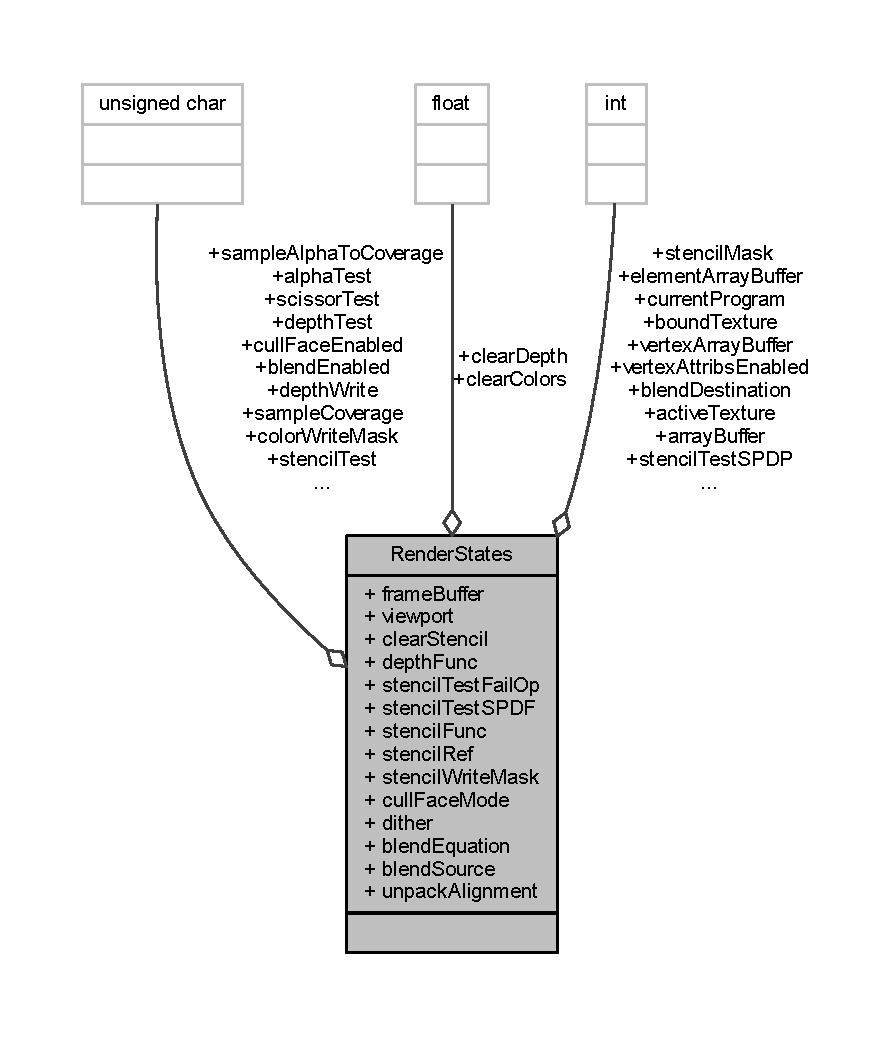
\includegraphics[width=350pt]{struct_render_states__coll__graph}
\end{center}
\end{figure}
\subsection*{Public Attributes}
\begin{DoxyCompactItemize}
\item 
\hypertarget{struct_render_states_a7c787f5a119727ff12a3b5e936b65dad}{int {\bfseries frame\-Buffer}}\label{struct_render_states_a7c787f5a119727ff12a3b5e936b65dad}

\item 
\hypertarget{struct_render_states_ae470d79c33f6223d353a5c5fd593e5bc}{int {\bfseries viewport} \mbox{[}4\mbox{]}}\label{struct_render_states_ae470d79c33f6223d353a5c5fd593e5bc}

\item 
\hypertarget{struct_render_states_ab5d6de94a08d0e76c91b4a0968919836}{float {\bfseries clear\-Colors} \mbox{[}4\mbox{]}}\label{struct_render_states_ab5d6de94a08d0e76c91b4a0968919836}

\item 
\hypertarget{struct_render_states_a9c7fde026031c0d14c046e6b330b5928}{float {\bfseries clear\-Depth}}\label{struct_render_states_a9c7fde026031c0d14c046e6b330b5928}

\item 
\hypertarget{struct_render_states_ad10edc9980c52c19c15f8bbe49b83058}{int {\bfseries clear\-Stencil}}\label{struct_render_states_ad10edc9980c52c19c15f8bbe49b83058}

\item 
\hypertarget{struct_render_states_a92f1526e7f826662ffa2e836d69c2f88}{unsigned char {\bfseries alpha\-Test}}\label{struct_render_states_a92f1526e7f826662ffa2e836d69c2f88}

\item 
\hypertarget{struct_render_states_af55a3d2f75c043b39567e6e21ee9c9d7}{unsigned char {\bfseries depth\-Test}}\label{struct_render_states_af55a3d2f75c043b39567e6e21ee9c9d7}

\item 
\hypertarget{struct_render_states_a3afe9d2c269f10f99fc7fe3cd4c3b826}{unsigned char {\bfseries depth\-Write}}\label{struct_render_states_a3afe9d2c269f10f99fc7fe3cd4c3b826}

\item 
\hypertarget{struct_render_states_a9a534b31746a6dabedd842824e3e783f}{int {\bfseries depth\-Func}}\label{struct_render_states_a9a534b31746a6dabedd842824e3e783f}

\item 
\hypertarget{struct_render_states_abd2afacd1b303bca14ba99c8ac8dbc3b}{unsigned char {\bfseries stencil\-Test}}\label{struct_render_states_abd2afacd1b303bca14ba99c8ac8dbc3b}

\item 
\hypertarget{struct_render_states_a0fbb13728e674f524b80253c36610558}{int {\bfseries stencil\-Test\-Fail\-Op}}\label{struct_render_states_a0fbb13728e674f524b80253c36610558}

\item 
\hypertarget{struct_render_states_ab9bb55980fb97152e6d48912c45cb18f}{int {\bfseries stencil\-Test\-S\-P\-D\-F}}\label{struct_render_states_ab9bb55980fb97152e6d48912c45cb18f}

\item 
\hypertarget{struct_render_states_a720241bcc4332f1f8603abb37efcddd1}{int {\bfseries stencil\-Test\-S\-P\-D\-P}}\label{struct_render_states_a720241bcc4332f1f8603abb37efcddd1}

\item 
\hypertarget{struct_render_states_a217dcbddffa2bee7b9b3415d69d798e3}{int {\bfseries stencil\-Func}}\label{struct_render_states_a217dcbddffa2bee7b9b3415d69d798e3}

\item 
\hypertarget{struct_render_states_a8528dd88cc0a21d725671c623cc9047c}{int {\bfseries stencil\-Ref}}\label{struct_render_states_a8528dd88cc0a21d725671c623cc9047c}

\item 
\hypertarget{struct_render_states_a082e1f854a68648e939c115fef7327d1}{unsigned int {\bfseries stencil\-Mask}}\label{struct_render_states_a082e1f854a68648e939c115fef7327d1}

\item 
\hypertarget{struct_render_states_ae4250f53fb7b6cca8787240bb1443f50}{unsigned int {\bfseries stencil\-Write\-Mask}}\label{struct_render_states_ae4250f53fb7b6cca8787240bb1443f50}

\item 
\hypertarget{struct_render_states_a4dfb0e96690840257885f23cfc8b84af}{unsigned char {\bfseries scissor\-Test}}\label{struct_render_states_a4dfb0e96690840257885f23cfc8b84af}

\item 
\hypertarget{struct_render_states_a21c1af780dd02e6ee6135cfd79512714}{unsigned char {\bfseries cull\-Face\-Enabled}}\label{struct_render_states_a21c1af780dd02e6ee6135cfd79512714}

\item 
\hypertarget{struct_render_states_ae00d6b29bf16812814d5322f6399afb3}{int {\bfseries cull\-Face\-Mode}}\label{struct_render_states_ae00d6b29bf16812814d5322f6399afb3}

\item 
\hypertarget{struct_render_states_a71b6832afc5e4593442f6c59ee9a7725}{unsigned char {\bfseries dither}}\label{struct_render_states_a71b6832afc5e4593442f6c59ee9a7725}

\item 
\hypertarget{struct_render_states_af734fdc472ec1288de5ff72b3639f457}{unsigned char {\bfseries sample\-Alpha\-To\-Coverage}}\label{struct_render_states_af734fdc472ec1288de5ff72b3639f457}

\item 
\hypertarget{struct_render_states_ab85a1a6f42f9b856f136bdf456e8d08c}{unsigned char {\bfseries sample\-Coverage}}\label{struct_render_states_ab85a1a6f42f9b856f136bdf456e8d08c}

\item 
\hypertarget{struct_render_states_a85a29b560f1a5e5be5012e8bbac9b729}{unsigned char {\bfseries blend\-Enabled}}\label{struct_render_states_a85a29b560f1a5e5be5012e8bbac9b729}

\item 
\hypertarget{struct_render_states_adbee0d395b078911dd49d5d7fd6c744f}{int {\bfseries blend\-Equation}}\label{struct_render_states_adbee0d395b078911dd49d5d7fd6c744f}

\item 
\hypertarget{struct_render_states_ac0cae6096b5454e685815edf1c41f188}{int {\bfseries blend\-Source}}\label{struct_render_states_ac0cae6096b5454e685815edf1c41f188}

\item 
\hypertarget{struct_render_states_abb72577e5e83fc705103a4192ecb3da1}{int {\bfseries blend\-Destination}}\label{struct_render_states_abb72577e5e83fc705103a4192ecb3da1}

\item 
\hypertarget{struct_render_states_ae9465ac804ffa406565da01b3b189ada}{unsigned char {\bfseries color\-Write\-Mask} \mbox{[}4\mbox{]}}\label{struct_render_states_ae9465ac804ffa406565da01b3b189ada}

\item 
\hypertarget{struct_render_states_a0ce45ab772961df0a1bf382017a7c198}{unsigned int {\bfseries array\-Buffer}}\label{struct_render_states_a0ce45ab772961df0a1bf382017a7c198}

\item 
\hypertarget{struct_render_states_ae0c2efdc0ff5c46bbffda94452682b82}{int {\bfseries vertex\-Attribs\-Enabled} \mbox{[}6\mbox{]}}\label{struct_render_states_ae0c2efdc0ff5c46bbffda94452682b82}

\item 
\hypertarget{struct_render_states_a36935647896a1f931c94c7c50df9bb49}{int {\bfseries active\-Texture}}\label{struct_render_states_a36935647896a1f931c94c7c50df9bb49}

\item 
\hypertarget{struct_render_states_a1051e8303f7175ca335f7276b1e7e41a}{unsigned int {\bfseries element\-Array\-Buffer}}\label{struct_render_states_a1051e8303f7175ca335f7276b1e7e41a}

\item 
\hypertarget{struct_render_states_a288f0d960627c83f3ac6318f2d689aca}{unsigned int {\bfseries vertex\-Array\-Buffer}}\label{struct_render_states_a288f0d960627c83f3ac6318f2d689aca}

\item 
\hypertarget{struct_render_states_a006e0d5c355695955a9ddef85846aa80}{int {\bfseries bound\-Texture} \mbox{[}4\mbox{]}}\label{struct_render_states_a006e0d5c355695955a9ddef85846aa80}

\item 
\hypertarget{struct_render_states_af269015f238dbdfd02643695f16cc749}{int {\bfseries current\-Program}}\label{struct_render_states_af269015f238dbdfd02643695f16cc749}

\item 
\hypertarget{struct_render_states_a8f8e59b92445cb2e7787be6734167c8d}{int {\bfseries unpack\-Alignment}}\label{struct_render_states_a8f8e59b92445cb2e7787be6734167c8d}

\end{DoxyCompactItemize}


The documentation for this struct was generated from the following file\-:\begin{DoxyCompactItemize}
\item 
Integration/\-U\-I/Render\-States.\-h\end{DoxyCompactItemize}

\hypertarget{class_u_i_renderer}{\section{U\-I\-Renderer Class Reference}
\label{class_u_i_renderer}\index{U\-I\-Renderer@{U\-I\-Renderer}}
}


X\-A\-M\-L Renderer.  




{\ttfamily \#include $<$U\-I\-Renderer.\-h$>$}



Collaboration diagram for U\-I\-Renderer\-:
\nopagebreak
\begin{figure}[H]
\begin{center}
\leavevmode
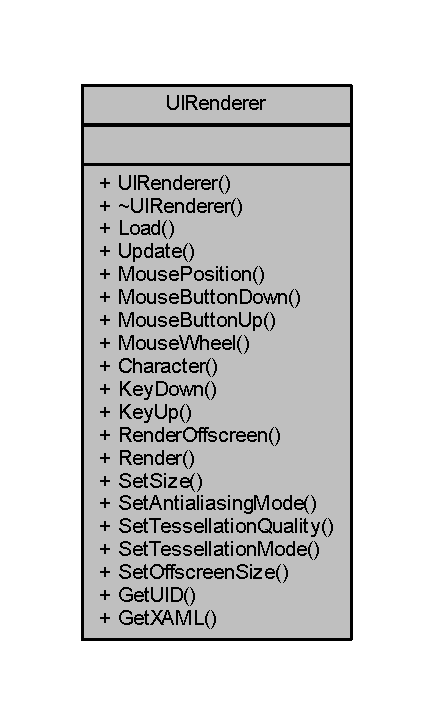
\includegraphics[width=350pt]{class_u_i_renderer__coll__graph}
\end{center}
\end{figure}
\subsection*{Public Member Functions}
\begin{DoxyCompactItemize}
\item 
\hypertarget{class_u_i_renderer_a8e0fb11ab4e123f3524756e276199351}{\hyperlink{class_u_i_renderer_a8e0fb11ab4e123f3524756e276199351}{U\-I\-Renderer} (const int id)}\label{class_u_i_renderer_a8e0fb11ab4e123f3524756e276199351}

\begin{DoxyCompactList}\small\item\em Creates a new \hyperlink{class_u_i_renderer}{U\-I\-Renderer}. \end{DoxyCompactList}\item 
void \hyperlink{class_u_i_renderer_a8e61394cd4b9dcf2242f1ec47e95ba5d}{Load} (std\-::string \hyperlink{class_u_i_renderer_ad9cc0fe1fcbf5e5182f7a18045c4ec07}{xaml}, std\-::string resource=\char`\"{}\char`\"{})
\begin{DoxyCompactList}\small\item\em Loads the specified xaml. \end{DoxyCompactList}\item 
void \hyperlink{class_u_i_renderer_a9304bf4f0ff00a671cf45ac5a4198004}{Update} (const double time)
\begin{DoxyCompactList}\small\item\em Update Renderer. \end{DoxyCompactList}\item 
\hypertarget{class_u_i_renderer_a305ee68738d0b1b833b73a85ca077261}{void \hyperlink{class_u_i_renderer_a305ee68738d0b1b833b73a85ca077261}{Mouse\-Position} (const int x, const int y)}\label{class_u_i_renderer_a305ee68738d0b1b833b73a85ca077261}

\begin{DoxyCompactList}\small\item\em Notifies the renderer that the mouse position has changed. \end{DoxyCompactList}\item 
\hypertarget{class_u_i_renderer_aad758939d86e2741ed7330252cfe3b74}{void \hyperlink{class_u_i_renderer_aad758939d86e2741ed7330252cfe3b74}{Mouse\-Button\-Down} (const int button)}\label{class_u_i_renderer_aad758939d86e2741ed7330252cfe3b74}

\begin{DoxyCompactList}\small\item\em Notifies the renderer that a mouse button has been pressed. \end{DoxyCompactList}\item 
\hypertarget{class_u_i_renderer_a9d72b10f66816ecb07c51025130591bf}{void \hyperlink{class_u_i_renderer_a9d72b10f66816ecb07c51025130591bf}{Mouse\-Button\-Up} (const int button)}\label{class_u_i_renderer_a9d72b10f66816ecb07c51025130591bf}

\begin{DoxyCompactList}\small\item\em Notifies the renderer that a mouse button has been released. \end{DoxyCompactList}\item 
\hypertarget{class_u_i_renderer_a02a32cecd924b8a855bce495672f8e4e}{void \hyperlink{class_u_i_renderer_a02a32cecd924b8a855bce495672f8e4e}{Mouse\-Wheel} (const int rotation)}\label{class_u_i_renderer_a02a32cecd924b8a855bce495672f8e4e}

\begin{DoxyCompactList}\small\item\em Notifies the renderer that the mouse wheel has been rotated. \end{DoxyCompactList}\item 
\hypertarget{class_u_i_renderer_ac6c071a178d51415329bf4f4f71dfd48}{void \hyperlink{class_u_i_renderer_ac6c071a178d51415329bf4f4f71dfd48}{Character} (const char character)}\label{class_u_i_renderer_ac6c071a178d51415329bf4f4f71dfd48}

\begin{DoxyCompactList}\small\item\em Sends the specified key to the renderer. \end{DoxyCompactList}\item 
\hypertarget{class_u_i_renderer_af0f5ee9edad9a7a35b46187d3fb697ea}{void \hyperlink{class_u_i_renderer_af0f5ee9edad9a7a35b46187d3fb697ea}{Key\-Down} (const int key)}\label{class_u_i_renderer_af0f5ee9edad9a7a35b46187d3fb697ea}

\begin{DoxyCompactList}\small\item\em Notifies renderer that a key was pressed. \end{DoxyCompactList}\item 
\hypertarget{class_u_i_renderer_acf25d6ac3df945fde9054c34bf28edd1}{void \hyperlink{class_u_i_renderer_acf25d6ac3df945fde9054c34bf28edd1}{Key\-Up} (const int key)}\label{class_u_i_renderer_acf25d6ac3df945fde9054c34bf28edd1}

\begin{DoxyCompactList}\small\item\em Notifies renderer that a key was released. \end{DoxyCompactList}\item 
\hypertarget{class_u_i_renderer_a1299a480654f95b593f1b22117e2324a}{void \hyperlink{class_u_i_renderer_a1299a480654f95b593f1b22117e2324a}{Render\-Offscreen} ()}\label{class_u_i_renderer_a1299a480654f95b593f1b22117e2324a}

\begin{DoxyCompactList}\small\item\em Render xaml offscreen. \end{DoxyCompactList}\item 
\hypertarget{class_u_i_renderer_a6961b53c2f5bf48d18c5164aaf5785d6}{void \hyperlink{class_u_i_renderer_a6961b53c2f5bf48d18c5164aaf5785d6}{Render} ()}\label{class_u_i_renderer_a6961b53c2f5bf48d18c5164aaf5785d6}

\begin{DoxyCompactList}\small\item\em Render xaml to screen. \end{DoxyCompactList}\item 
\hypertarget{class_u_i_renderer_a9afd9d07f2c93d426f55ce2e84a64cef}{void \hyperlink{class_u_i_renderer_a9afd9d07f2c93d426f55ce2e84a64cef}{Set\-Size} (const int width, const int height)}\label{class_u_i_renderer_a9afd9d07f2c93d426f55ce2e84a64cef}

\begin{DoxyCompactList}\small\item\em Sets the renderer to the specified size. \end{DoxyCompactList}\item 
void \hyperlink{class_u_i_renderer_a05d5fed9d98c02a150efeb8e6ea36812}{Set\-Antialiasing\-Mode} (const int mode)
\begin{DoxyCompactList}\small\item\em Sets the antialiasing mode. \end{DoxyCompactList}\item 
void \hyperlink{class_u_i_renderer_a77ab17ad59e589eb32d55699ea1ab1c6}{Set\-Tessellation\-Quality} (const int quality)
\begin{DoxyCompactList}\small\item\em Sets the tesselation quality. \end{DoxyCompactList}\item 
void \hyperlink{class_u_i_renderer_a54d4d9236175ecca2568dffa8f6a60e6}{Set\-Tessellation\-Mode} (const int mode)
\begin{DoxyCompactList}\small\item\em Sets the tesselation mode. \end{DoxyCompactList}\item 
void \hyperlink{class_u_i_renderer_ad8eacb018b912e5d7786ca6f1642b4ce}{Set\-Offscreen\-Size} (const int width, const int height, const int multisample)
\begin{DoxyCompactList}\small\item\em Set offscreen rendering quality. \end{DoxyCompactList}\item 
int \hyperlink{class_u_i_renderer_a45454e14885545c166a795d4a0884a38}{Get\-U\-I\-D} ()
\begin{DoxyCompactList}\small\item\em Returns the renderers uid. \end{DoxyCompactList}\item 
Noesis\-::\-Gui\-::\-Framework\-Element $\ast$ \hyperlink{class_u_i_renderer_a0989015bf54f7b6c624829c1fbf284d7}{Get\-X\-A\-M\-L} ()
\begin{DoxyCompactList}\small\item\em Returns the loaded X\-A\-M\-L. \end{DoxyCompactList}\item 
void \hyperlink{class_u_i_renderer_af9dca433a7bba7349412539760e9a6d6}{Set\-Flags} (const int flags)
\begin{DoxyCompactList}\small\item\em Sets renderer flags. \end{DoxyCompactList}\end{DoxyCompactItemize}
\subsection*{Static Public Attributes}
\begin{DoxyCompactItemize}
\item 
\hypertarget{class_u_i_renderer_a6472e56938d0e576e6e49f55f53355d1}{static const int {\bfseries Wireframe} = 1}\label{class_u_i_renderer_a6472e56938d0e576e6e49f55f53355d1}

\item 
\hypertarget{class_u_i_renderer_a1936b4d333e8b4dcbfc8ae7842d7831b}{static const int {\bfseries Color\-Batch} = 2}\label{class_u_i_renderer_a1936b4d333e8b4dcbfc8ae7842d7831b}

\item 
\hypertarget{class_u_i_renderer_a063e1e52cf61320266f44049db712ed5}{static const int {\bfseries Overdraw} = 4}\label{class_u_i_renderer_a063e1e52cf61320266f44049db712ed5}

\item 
\hypertarget{class_u_i_renderer_a0b81268994fe6323c3489d148d9c2a69}{static const int {\bfseries Flip\-Y} = 8}\label{class_u_i_renderer_a0b81268994fe6323c3489d148d9c2a69}

\end{DoxyCompactItemize}
\subsection*{Private Attributes}
\begin{DoxyCompactItemize}
\item 
\hypertarget{class_u_i_renderer_a191e33b40b855c04117de4d49d48e99b}{int \hyperlink{class_u_i_renderer_a191e33b40b855c04117de4d49d48e99b}{uid}}\label{class_u_i_renderer_a191e33b40b855c04117de4d49d48e99b}

\begin{DoxyCompactList}\small\item\em Unique id. \end{DoxyCompactList}\item 
\hypertarget{class_u_i_renderer_a44cffd1da636ee3d5a03ebee3e880d26}{\hyperlink{class_open_g_l_state}{Open\-G\-L\-State} $\ast$ \hyperlink{class_u_i_renderer_a44cffd1da636ee3d5a03ebee3e880d26}{gl\-State}}\label{class_u_i_renderer_a44cffd1da636ee3d5a03ebee3e880d26}

\begin{DoxyCompactList}\small\item\em Open\-G\-L state. \end{DoxyCompactList}\item 
\hypertarget{class_u_i_renderer_ab365eca2491514a80282a621626920d6}{Leadwerks\-::\-Vec3 \hyperlink{class_u_i_renderer_ab365eca2491514a80282a621626920d6}{mspos}}\label{class_u_i_renderer_ab365eca2491514a80282a621626920d6}

\begin{DoxyCompactList}\small\item\em Last known mouse position. \end{DoxyCompactList}\item 
\hypertarget{class_u_i_renderer_a9f78449d8d996e66f1e1d75c3cd6276f}{Noesis\-::\-Gui\-::\-I\-Renderer $\ast$ \hyperlink{class_u_i_renderer_a9f78449d8d996e66f1e1d75c3cd6276f}{renderer}}\label{class_u_i_renderer_a9f78449d8d996e66f1e1d75c3cd6276f}

\begin{DoxyCompactList}\small\item\em Actual renderer. \end{DoxyCompactList}\item 
\hypertarget{class_u_i_renderer_ad9cc0fe1fcbf5e5182f7a18045c4ec07}{Noesis\-::\-Gui\-::\-Framework\-Element $\ast$ \hyperlink{class_u_i_renderer_ad9cc0fe1fcbf5e5182f7a18045c4ec07}{xaml}}\label{class_u_i_renderer_ad9cc0fe1fcbf5e5182f7a18045c4ec07}

\begin{DoxyCompactList}\small\item\em Loaded xaml. \end{DoxyCompactList}\end{DoxyCompactItemize}


\subsection{Detailed Description}
X\-A\-M\-L Renderer. 

\subsection{Member Function Documentation}
\hypertarget{class_u_i_renderer_a45454e14885545c166a795d4a0884a38}{\index{U\-I\-Renderer@{U\-I\-Renderer}!Get\-U\-I\-D@{Get\-U\-I\-D}}
\index{Get\-U\-I\-D@{Get\-U\-I\-D}!UIRenderer@{U\-I\-Renderer}}
\subsubsection[{Get\-U\-I\-D}]{\setlength{\rightskip}{0pt plus 5cm}int U\-I\-Renderer\-::\-Get\-U\-I\-D (
\begin{DoxyParamCaption}
{}
\end{DoxyParamCaption}
)\hspace{0.3cm}{\ttfamily [inline]}}}\label{class_u_i_renderer_a45454e14885545c166a795d4a0884a38}


Returns the renderers uid. 

\begin{DoxyReturn}{Returns}
uid 
\end{DoxyReturn}
\hypertarget{class_u_i_renderer_a0989015bf54f7b6c624829c1fbf284d7}{\index{U\-I\-Renderer@{U\-I\-Renderer}!Get\-X\-A\-M\-L@{Get\-X\-A\-M\-L}}
\index{Get\-X\-A\-M\-L@{Get\-X\-A\-M\-L}!UIRenderer@{U\-I\-Renderer}}
\subsubsection[{Get\-X\-A\-M\-L}]{\setlength{\rightskip}{0pt plus 5cm}Noesis\-::\-Gui\-::\-Framework\-Element $\ast$ U\-I\-Renderer\-::\-Get\-X\-A\-M\-L (
\begin{DoxyParamCaption}
{}
\end{DoxyParamCaption}
)}}\label{class_u_i_renderer_a0989015bf54f7b6c624829c1fbf284d7}


Returns the loaded X\-A\-M\-L. 

\begin{DoxyReturn}{Returns}
X\-A\-M\-L 
\end{DoxyReturn}
\hypertarget{class_u_i_renderer_a8e61394cd4b9dcf2242f1ec47e95ba5d}{\index{U\-I\-Renderer@{U\-I\-Renderer}!Load@{Load}}
\index{Load@{Load}!UIRenderer@{U\-I\-Renderer}}
\subsubsection[{Load}]{\setlength{\rightskip}{0pt plus 5cm}void U\-I\-Renderer\-::\-Load (
\begin{DoxyParamCaption}
\item[{std\-::string}]{xaml, }
\item[{std\-::string}]{resource = {\ttfamily \char`\"{}\char`\"{}}}
\end{DoxyParamCaption}
)}}\label{class_u_i_renderer_a8e61394cd4b9dcf2242f1ec47e95ba5d}


Loads the specified xaml. 


\begin{DoxyParams}[1]{Parameters}
\mbox{\tt in}  & {\em xaml} & X\-A\-M\-L to load \\
\hline
\mbox{\tt in}  & {\em resource} & Additional xaml style / resource \\
\hline
\end{DoxyParams}
\hypertarget{class_u_i_renderer_a05d5fed9d98c02a150efeb8e6ea36812}{\index{U\-I\-Renderer@{U\-I\-Renderer}!Set\-Antialiasing\-Mode@{Set\-Antialiasing\-Mode}}
\index{Set\-Antialiasing\-Mode@{Set\-Antialiasing\-Mode}!UIRenderer@{U\-I\-Renderer}}
\subsubsection[{Set\-Antialiasing\-Mode}]{\setlength{\rightskip}{0pt plus 5cm}void U\-I\-Renderer\-::\-Set\-Antialiasing\-Mode (
\begin{DoxyParamCaption}
\item[{const int}]{mode}
\end{DoxyParamCaption}
)}}\label{class_u_i_renderer_a05d5fed9d98c02a150efeb8e6ea36812}


Sets the antialiasing mode. 

Default value is M\-S\-A\-A. 
\begin{DoxyParams}[1]{Parameters}
\mbox{\tt in}  & {\em mode} & Noesis\-::\-Gui\-::\-Antialiasing\-Mode \\
\hline
\end{DoxyParams}
\hypertarget{class_u_i_renderer_af9dca433a7bba7349412539760e9a6d6}{\index{U\-I\-Renderer@{U\-I\-Renderer}!Set\-Flags@{Set\-Flags}}
\index{Set\-Flags@{Set\-Flags}!UIRenderer@{U\-I\-Renderer}}
\subsubsection[{Set\-Flags}]{\setlength{\rightskip}{0pt plus 5cm}void U\-I\-Renderer\-::\-Set\-Flags (
\begin{DoxyParamCaption}
\item[{const int}]{flags}
\end{DoxyParamCaption}
)}}\label{class_u_i_renderer_af9dca433a7bba7349412539760e9a6d6}


Sets renderer flags. 

Noesis\-::\-Gui\-::\-Renderer\-Flags 
\begin{DoxyParams}[1]{Parameters}
\mbox{\tt in}  & {\em flag} & Wireframe, Color\-Batch, Overdraw or Flip\-Y. Flags can be combined. \\
\hline
\end{DoxyParams}
\hypertarget{class_u_i_renderer_ad8eacb018b912e5d7786ca6f1642b4ce}{\index{U\-I\-Renderer@{U\-I\-Renderer}!Set\-Offscreen\-Size@{Set\-Offscreen\-Size}}
\index{Set\-Offscreen\-Size@{Set\-Offscreen\-Size}!UIRenderer@{U\-I\-Renderer}}
\subsubsection[{Set\-Offscreen\-Size}]{\setlength{\rightskip}{0pt plus 5cm}void U\-I\-Renderer\-::\-Set\-Offscreen\-Size (
\begin{DoxyParamCaption}
\item[{const int}]{width, }
\item[{const int}]{height, }
\item[{const int}]{multisample}
\end{DoxyParamCaption}
)}}\label{class_u_i_renderer_ad8eacb018b912e5d7786ca6f1642b4ce}


Set offscreen rendering quality. 

By default, offscreen textures have the same dimensions that the target surface and multisampling is disabled for them. 
\begin{DoxyParams}[1]{Parameters}
\mbox{\tt in}  & {\em width} & Relative width (0-\/1) \\
\hline
\mbox{\tt in}  & {\em height} & Relative height (0-\/1) \\
\hline
\mbox{\tt in}  & {\em multisample} & Noesis\-::\-Render\-::\-Multi\-Sample \\
\hline
\end{DoxyParams}
\hypertarget{class_u_i_renderer_a54d4d9236175ecca2568dffa8f6a60e6}{\index{U\-I\-Renderer@{U\-I\-Renderer}!Set\-Tessellation\-Mode@{Set\-Tessellation\-Mode}}
\index{Set\-Tessellation\-Mode@{Set\-Tessellation\-Mode}!UIRenderer@{U\-I\-Renderer}}
\subsubsection[{Set\-Tessellation\-Mode}]{\setlength{\rightskip}{0pt plus 5cm}void U\-I\-Renderer\-::\-Set\-Tessellation\-Mode (
\begin{DoxyParamCaption}
\item[{const int}]{mode}
\end{DoxyParamCaption}
)}}\label{class_u_i_renderer_a54d4d9236175ecca2568dffa8f6a60e6}


Sets the tesselation mode. 

Default value is Threshold. 
\begin{DoxyParams}[1]{Parameters}
\mbox{\tt in}  & {\em mode} & Noesis\-::\-Gui\-::\-Tessellation\-Mode \\
\hline
\end{DoxyParams}
\hypertarget{class_u_i_renderer_a77ab17ad59e589eb32d55699ea1ab1c6}{\index{U\-I\-Renderer@{U\-I\-Renderer}!Set\-Tessellation\-Quality@{Set\-Tessellation\-Quality}}
\index{Set\-Tessellation\-Quality@{Set\-Tessellation\-Quality}!UIRenderer@{U\-I\-Renderer}}
\subsubsection[{Set\-Tessellation\-Quality}]{\setlength{\rightskip}{0pt plus 5cm}void U\-I\-Renderer\-::\-Set\-Tessellation\-Quality (
\begin{DoxyParamCaption}
\item[{const int}]{quality}
\end{DoxyParamCaption}
)}}\label{class_u_i_renderer_a77ab17ad59e589eb32d55699ea1ab1c6}


Sets the tesselation quality. 

Default value is Medium. 
\begin{DoxyParams}[1]{Parameters}
\mbox{\tt in}  & {\em quality} & Noesis\-::\-Gui\-::\-Tessellation\-Quality \\
\hline
\end{DoxyParams}
\hypertarget{class_u_i_renderer_a9304bf4f0ff00a671cf45ac5a4198004}{\index{U\-I\-Renderer@{U\-I\-Renderer}!Update@{Update}}
\index{Update@{Update}!UIRenderer@{U\-I\-Renderer}}
\subsubsection[{Update}]{\setlength{\rightskip}{0pt plus 5cm}void U\-I\-Renderer\-::\-Update (
\begin{DoxyParamCaption}
\item[{const double}]{time}
\end{DoxyParamCaption}
)}}\label{class_u_i_renderer_a9304bf4f0ff00a671cf45ac5a4198004}


Update Renderer. 

Updates the noesis kernel, the renderer and the render\-Commands. 
\begin{DoxyParams}[1]{Parameters}
\mbox{\tt in}  & {\em time} & Time in s \\
\hline
\end{DoxyParams}


The documentation for this class was generated from the following files\-:\begin{DoxyCompactItemize}
\item 
Integration/\-U\-I/U\-I\-Renderer.\-h\item 
Integration/\-U\-I/U\-I\-Renderer.\-cpp\end{DoxyCompactItemize}

\hypertarget{class_u_i_render_target}{\section{U\-I\-Render\-Target Class Reference}
\label{class_u_i_render_target}\index{U\-I\-Render\-Target@{U\-I\-Render\-Target}}
}


Render target.  




{\ttfamily \#include $<$U\-I\-Render\-Target.\-h$>$}



Collaboration diagram for U\-I\-Render\-Target\-:\nopagebreak
\begin{figure}[H]
\begin{center}
\leavevmode
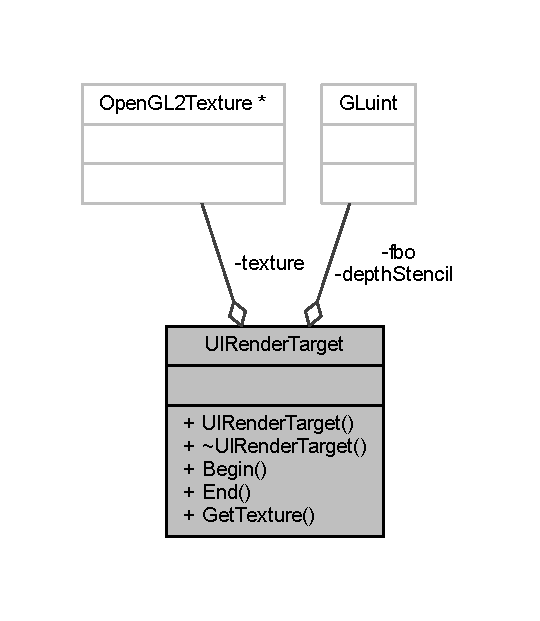
\includegraphics[width=259pt]{class_u_i_render_target__coll__graph}
\end{center}
\end{figure}
\subsection*{Public Member Functions}
\begin{DoxyCompactItemize}
\item 
\hyperlink{class_u_i_render_target_a0a92fb5e803c91ca4288b4244ab6af3b}{U\-I\-Render\-Target} (const int width, const int height, const int format=Leadwerks\-::\-Texture\-::\-R\-G\-B\-A, const int flags=0, const int frames=1, const int samples=0)
\begin{DoxyCompactList}\small\item\em Craetes a new render target. \end{DoxyCompactList}\item 
\hypertarget{class_u_i_render_target_a647cc3a9d76dca037954d2c694dc8499}{void \hyperlink{class_u_i_render_target_a647cc3a9d76dca037954d2c694dc8499}{Begin} ()}\label{class_u_i_render_target_a647cc3a9d76dca037954d2c694dc8499}

\begin{DoxyCompactList}\small\item\em Start rendering into the render target. \end{DoxyCompactList}\item 
\hypertarget{class_u_i_render_target_ab660bf14c0e070939943076825e859cb}{void \hyperlink{class_u_i_render_target_ab660bf14c0e070939943076825e859cb}{End} ()}\label{class_u_i_render_target_ab660bf14c0e070939943076825e859cb}

\begin{DoxyCompactList}\small\item\em Stop rendering into the render target. \end{DoxyCompactList}\item 
Leadwerks\-::\-Texture $\ast$ \hyperlink{class_u_i_render_target_a6ede8013f6b4c87556c37f086f1a864d}{Get\-Texture} ()
\begin{DoxyCompactList}\small\item\em Get render target texture. \end{DoxyCompactList}\end{DoxyCompactItemize}
\subsection*{Private Attributes}
\begin{DoxyCompactItemize}
\item 
\hypertarget{class_u_i_render_target_a71089abfab0c5ef2e04fc81bbc986ebf}{G\-Luint \hyperlink{class_u_i_render_target_a71089abfab0c5ef2e04fc81bbc986ebf}{fbo}}\label{class_u_i_render_target_a71089abfab0c5ef2e04fc81bbc986ebf}

\begin{DoxyCompactList}\small\item\em Framebuffer. \end{DoxyCompactList}\item 
\hypertarget{class_u_i_render_target_a59c466d2b55a013e36dbff39dda3a38f}{G\-Luint \hyperlink{class_u_i_render_target_a59c466d2b55a013e36dbff39dda3a38f}{depth\-Stencil}}\label{class_u_i_render_target_a59c466d2b55a013e36dbff39dda3a38f}

\begin{DoxyCompactList}\small\item\em Renderbuffer. \end{DoxyCompactList}\item 
\hypertarget{class_u_i_render_target_ae865daebacafba6e779ab2dec1c04690}{Leadwerks\-::\-Open\-G\-L2\-Texture $\ast$ \hyperlink{class_u_i_render_target_ae865daebacafba6e779ab2dec1c04690}{texture}}\label{class_u_i_render_target_ae865daebacafba6e779ab2dec1c04690}

\begin{DoxyCompactList}\small\item\em Texture. \end{DoxyCompactList}\end{DoxyCompactItemize}


\subsection{Detailed Description}
Render target. 

Creates a new F\-B\-O with stencil enabled in the current Open\-G\-L context. 

\subsection{Constructor \& Destructor Documentation}
\hypertarget{class_u_i_render_target_a0a92fb5e803c91ca4288b4244ab6af3b}{\index{U\-I\-Render\-Target@{U\-I\-Render\-Target}!U\-I\-Render\-Target@{U\-I\-Render\-Target}}
\index{U\-I\-Render\-Target@{U\-I\-Render\-Target}!UIRenderTarget@{U\-I\-Render\-Target}}
\subsubsection[{U\-I\-Render\-Target}]{\setlength{\rightskip}{0pt plus 5cm}U\-I\-Render\-Target\-::\-U\-I\-Render\-Target (
\begin{DoxyParamCaption}
\item[{const int}]{width, }
\item[{const int}]{height, }
\item[{const int}]{format = {\ttfamily Leadwerks\-:\-:Texture\-:\-:RGBA}, }
\item[{const int}]{flags = {\ttfamily 0}, }
\item[{const int}]{frames = {\ttfamily 1}, }
\item[{const int}]{samples = {\ttfamily 0}}
\end{DoxyParamCaption}
)}}\label{class_u_i_render_target_a0a92fb5e803c91ca4288b4244ab6af3b}


Craetes a new render target. 

Parameter information\-: \href{http://www.leadwerks.com/werkspace/page/documentation/_/command-reference/texture/texturecreate-r340}{\tt http\-://www.\-leadwerks.\-com/werkspace/page/documentation/\-\_\-/command-\/reference/texture/texturecreate-\/r340} 
\begin{DoxyParams}[1]{Parameters}
\mbox{\tt in}  & {\em width} & Texture width \\
\hline
\mbox{\tt in}  & {\em height} & Texture height \\
\hline
\mbox{\tt in}  & {\em format} & Texture format \\
\hline
\mbox{\tt in}  & {\em flags} & Texture flags \\
\hline
\mbox{\tt in}  & {\em frames} & Texture frames \\
\hline
\mbox{\tt in}  & {\em samples} & Texture samples \\
\hline
\end{DoxyParams}


\subsection{Member Function Documentation}
\hypertarget{class_u_i_render_target_a6ede8013f6b4c87556c37f086f1a864d}{\index{U\-I\-Render\-Target@{U\-I\-Render\-Target}!Get\-Texture@{Get\-Texture}}
\index{Get\-Texture@{Get\-Texture}!UIRenderTarget@{U\-I\-Render\-Target}}
\subsubsection[{Get\-Texture}]{\setlength{\rightskip}{0pt plus 5cm}Leadwerks\-::\-Texture $\ast$ U\-I\-Render\-Target\-::\-Get\-Texture (
\begin{DoxyParamCaption}
{}
\end{DoxyParamCaption}
)}}\label{class_u_i_render_target_a6ede8013f6b4c87556c37f086f1a864d}


Get render target texture. 

\begin{DoxyReturn}{Returns}
Texture 
\end{DoxyReturn}


The documentation for this class was generated from the following files\-:\begin{DoxyCompactItemize}
\item 
Integration/\-U\-I/U\-I\-Render\-Target.\-h\item 
Integration/\-U\-I/U\-I\-Render\-Target.\-cpp\end{DoxyCompactItemize}

\hypertarget{class_u_i_system}{\section{U\-I\-System Class Reference}
\label{class_u_i_system}\index{U\-I\-System@{U\-I\-System}}
}


Manages all U\-I related renderers.  




{\ttfamily \#include $<$U\-I\-System.\-h$>$}



Collaboration diagram for U\-I\-System\-:
\nopagebreak
\begin{figure}[H]
\begin{center}
\leavevmode
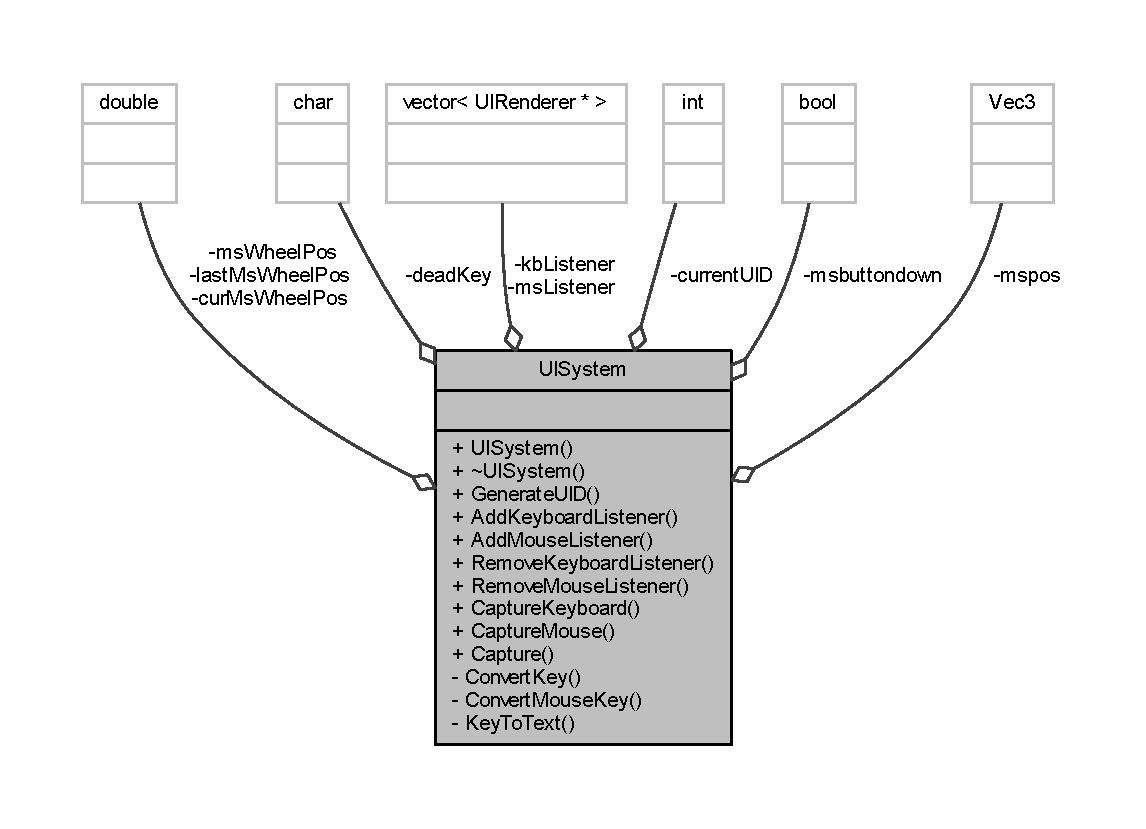
\includegraphics[width=350pt]{class_u_i_system__coll__graph}
\end{center}
\end{figure}
\subsection*{Public Member Functions}
\begin{DoxyCompactItemize}
\item 
\hypertarget{class_u_i_system_ac930744c42c305f09deacd176045392b}{\hyperlink{class_u_i_system_ac930744c42c305f09deacd176045392b}{U\-I\-System} ()}\label{class_u_i_system_ac930744c42c305f09deacd176045392b}

\begin{DoxyCompactList}\small\item\em Initializes noesis. \end{DoxyCompactList}\item 
int \hyperlink{class_u_i_system_a5735f001450f7ecd82a4de76558640c6}{Generate\-U\-I\-D} ()
\begin{DoxyCompactList}\small\item\em Generates a new unique id. \end{DoxyCompactList}\item 
void \hyperlink{class_u_i_system_a45a982a524c4d35a383232984062e21f}{Add\-Keyboard\-Listener} (\hyperlink{class_u_i_renderer}{U\-I\-Renderer} $\ast$\&ui\-Renderer)
\begin{DoxyCompactList}\small\item\em Registers a listener for keyboard input events. \end{DoxyCompactList}\item 
void \hyperlink{class_u_i_system_a51a64e1ed2767a9f57c52195468ea3bf}{Add\-Mouse\-Listener} (\hyperlink{class_u_i_renderer}{U\-I\-Renderer} $\ast$\&ui\-Renderer)
\begin{DoxyCompactList}\small\item\em Registers a listener for mouse input events. \end{DoxyCompactList}\item 
void \hyperlink{class_u_i_system_a01f185ae5eb2dd12607cff3fbaaebad2}{Remove\-Keyboard\-Listener} (const int uid)
\begin{DoxyCompactList}\small\item\em Removes a listener for keyboard input events. \end{DoxyCompactList}\item 
void \hyperlink{class_u_i_system_a833da0ec7454752a7872d82051366aad}{Remove\-Mouse\-Listener} (const int uid)
\begin{DoxyCompactList}\small\item\em Removes a listener for mouse input events. \end{DoxyCompactList}\item 
\hypertarget{class_u_i_system_a2dd00ec5f796185c5d7601ec03c29695}{void \hyperlink{class_u_i_system_a2dd00ec5f796185c5d7601ec03c29695}{Capture\-Keyboard} ()}\label{class_u_i_system_a2dd00ec5f796185c5d7601ec03c29695}

\begin{DoxyCompactList}\small\item\em Capture keyboard input. \end{DoxyCompactList}\item 
\hypertarget{class_u_i_system_a9139946c67db84d93b4a23a42a51eea1}{void \hyperlink{class_u_i_system_a9139946c67db84d93b4a23a42a51eea1}{Capture\-Mouse} ()}\label{class_u_i_system_a9139946c67db84d93b4a23a42a51eea1}

\begin{DoxyCompactList}\small\item\em Capture mouse input. \end{DoxyCompactList}\item 
\hypertarget{class_u_i_system_a29ac5727af1a979e24f4e8a92ff7a5a3}{void \hyperlink{class_u_i_system_a29ac5727af1a979e24f4e8a92ff7a5a3}{Capture} ()}\label{class_u_i_system_a29ac5727af1a979e24f4e8a92ff7a5a3}

\begin{DoxyCompactList}\small\item\em Capture Keyboard and mouse input. \end{DoxyCompactList}\end{DoxyCompactItemize}
\subsection*{Private Member Functions}
\begin{DoxyCompactItemize}
\item 
int \hyperlink{class_u_i_system_a609dfe50f7414f19e8fc6552807eb4e8}{Convert\-Key} (const int key)
\begin{DoxyCompactList}\small\item\em Convert Leadwerks V-\/\-Key to Noesis compatible key-\/code. \end{DoxyCompactList}\item 
int \hyperlink{class_u_i_system_aa6023e6a0d3b6ce665ae4eabb9ef34f7}{Convert\-Mouse\-Key} (const int key)
\begin{DoxyCompactList}\small\item\em Convert Leadwerks mouse-\/key to Noesis compatible key-\/code. \end{DoxyCompactList}\item 
int \hyperlink{class_u_i_system_ab10ce968219079f159b53a035e115cee}{Key\-To\-Text} (const int vkey)
\begin{DoxyCompactList}\small\item\em Converts a vkey to an ascii code. \end{DoxyCompactList}\end{DoxyCompactItemize}
\subsection*{Private Attributes}
\begin{DoxyCompactItemize}
\item 
\hypertarget{class_u_i_system_af9a599a508924e7949de438b95e2ed2f}{std\-::vector$<$ \hyperlink{class_u_i_renderer}{U\-I\-Renderer} $\ast$ $>$ \hyperlink{class_u_i_system_af9a599a508924e7949de438b95e2ed2f}{ms\-Listener}}\label{class_u_i_system_af9a599a508924e7949de438b95e2ed2f}

\begin{DoxyCompactList}\small\item\em Mouse listeners. \end{DoxyCompactList}\item 
\hypertarget{class_u_i_system_ae62a4dc19872c94de26957ccccec9112}{std\-::vector$<$ \hyperlink{class_u_i_renderer}{U\-I\-Renderer} $\ast$ $>$ \hyperlink{class_u_i_system_ae62a4dc19872c94de26957ccccec9112}{kb\-Listener}}\label{class_u_i_system_ae62a4dc19872c94de26957ccccec9112}

\begin{DoxyCompactList}\small\item\em Keyboard listeners. \end{DoxyCompactList}\item 
\hypertarget{class_u_i_system_afa67c850ac0fcebe6d5ce507c2b8fb0b}{int \hyperlink{class_u_i_system_afa67c850ac0fcebe6d5ce507c2b8fb0b}{current\-U\-I\-D}}\label{class_u_i_system_afa67c850ac0fcebe6d5ce507c2b8fb0b}

\begin{DoxyCompactList}\small\item\em Current unique id. \end{DoxyCompactList}\item 
\hypertarget{class_u_i_system_a56a33b6591efa7ee02df81c02c64e7d5}{char \hyperlink{class_u_i_system_a56a33b6591efa7ee02df81c02c64e7d5}{dead\-Key}}\label{class_u_i_system_a56a33b6591efa7ee02df81c02c64e7d5}

\begin{DoxyCompactList}\small\item\em Last found deadkey. \end{DoxyCompactList}\item 
\hypertarget{class_u_i_system_a4b44c8ec919f89201bd36f4652f28751}{bool \hyperlink{class_u_i_system_a4b44c8ec919f89201bd36f4652f28751}{msbuttondown} \mbox{[}5\mbox{]}}\label{class_u_i_system_a4b44c8ec919f89201bd36f4652f28751}

\begin{DoxyCompactList}\small\item\em Keydown state for all mouse buttons. \end{DoxyCompactList}\item 
\hypertarget{class_u_i_system_a43e14bcc1d98c5e8651cde6e194206d7}{Leadwerks\-::\-Vec3 \hyperlink{class_u_i_system_a43e14bcc1d98c5e8651cde6e194206d7}{mspos}}\label{class_u_i_system_a43e14bcc1d98c5e8651cde6e194206d7}

\begin{DoxyCompactList}\small\item\em Mouse position. \end{DoxyCompactList}\item 
\hypertarget{class_u_i_system_a7772c89c41305eddb51133916908a33d}{double {\bfseries last\-Ms\-Wheel\-Pos}}\label{class_u_i_system_a7772c89c41305eddb51133916908a33d}

\item 
\hypertarget{class_u_i_system_a73ad35f216be30560290a1870caf9c67}{double {\bfseries cur\-Ms\-Wheel\-Pos}}\label{class_u_i_system_a73ad35f216be30560290a1870caf9c67}

\item 
\hypertarget{class_u_i_system_aaf09f639ae523ee3d7ba186951518ec8}{double {\bfseries ms\-Wheel\-Pos}}\label{class_u_i_system_aaf09f639ae523ee3d7ba186951518ec8}

\end{DoxyCompactItemize}


\subsection{Detailed Description}
Manages all U\-I related renderers. 

Initializes all required noesis components and manages input for the U\-I\-Renderers. 

\subsection{Member Function Documentation}
\hypertarget{class_u_i_system_a45a982a524c4d35a383232984062e21f}{\index{U\-I\-System@{U\-I\-System}!Add\-Keyboard\-Listener@{Add\-Keyboard\-Listener}}
\index{Add\-Keyboard\-Listener@{Add\-Keyboard\-Listener}!UISystem@{U\-I\-System}}
\subsubsection[{Add\-Keyboard\-Listener}]{\setlength{\rightskip}{0pt plus 5cm}void U\-I\-System\-::\-Add\-Keyboard\-Listener (
\begin{DoxyParamCaption}
\item[{{\bf U\-I\-Renderer} $\ast$\&}]{ui\-Renderer}
\end{DoxyParamCaption}
)}}\label{class_u_i_system_a45a982a524c4d35a383232984062e21f}


Registers a listener for keyboard input events. 

\begin{DoxyWarning}{Warning}
The specified renderer must have an unique id assigned 
\end{DoxyWarning}

\begin{DoxyParams}[1]{Parameters}
\mbox{\tt in}  & {\em ui\-Renderer} & Listener \\
\hline
\end{DoxyParams}
\hypertarget{class_u_i_system_a51a64e1ed2767a9f57c52195468ea3bf}{\index{U\-I\-System@{U\-I\-System}!Add\-Mouse\-Listener@{Add\-Mouse\-Listener}}
\index{Add\-Mouse\-Listener@{Add\-Mouse\-Listener}!UISystem@{U\-I\-System}}
\subsubsection[{Add\-Mouse\-Listener}]{\setlength{\rightskip}{0pt plus 5cm}void U\-I\-System\-::\-Add\-Mouse\-Listener (
\begin{DoxyParamCaption}
\item[{{\bf U\-I\-Renderer} $\ast$\&}]{ui\-Renderer}
\end{DoxyParamCaption}
)}}\label{class_u_i_system_a51a64e1ed2767a9f57c52195468ea3bf}


Registers a listener for mouse input events. 

\begin{DoxyWarning}{Warning}
The specified renderer must have an unique id assigned 
\end{DoxyWarning}

\begin{DoxyParams}[1]{Parameters}
\mbox{\tt in}  & {\em ui\-Renderer} & Listener \\
\hline
\end{DoxyParams}
\hypertarget{class_u_i_system_a609dfe50f7414f19e8fc6552807eb4e8}{\index{U\-I\-System@{U\-I\-System}!Convert\-Key@{Convert\-Key}}
\index{Convert\-Key@{Convert\-Key}!UISystem@{U\-I\-System}}
\subsubsection[{Convert\-Key}]{\setlength{\rightskip}{0pt plus 5cm}int U\-I\-System\-::\-Convert\-Key (
\begin{DoxyParamCaption}
\item[{const int}]{key}
\end{DoxyParamCaption}
)\hspace{0.3cm}{\ttfamily [private]}}}\label{class_u_i_system_a609dfe50f7414f19e8fc6552807eb4e8}


Convert Leadwerks V-\/\-Key to Noesis compatible key-\/code. 

\begin{DoxyReturn}{Returns}
Noesis compatible key-\/code 
\end{DoxyReturn}
\hypertarget{class_u_i_system_aa6023e6a0d3b6ce665ae4eabb9ef34f7}{\index{U\-I\-System@{U\-I\-System}!Convert\-Mouse\-Key@{Convert\-Mouse\-Key}}
\index{Convert\-Mouse\-Key@{Convert\-Mouse\-Key}!UISystem@{U\-I\-System}}
\subsubsection[{Convert\-Mouse\-Key}]{\setlength{\rightskip}{0pt plus 5cm}int U\-I\-System\-::\-Convert\-Mouse\-Key (
\begin{DoxyParamCaption}
\item[{const int}]{key}
\end{DoxyParamCaption}
)\hspace{0.3cm}{\ttfamily [private]}}}\label{class_u_i_system_aa6023e6a0d3b6ce665ae4eabb9ef34f7}


Convert Leadwerks mouse-\/key to Noesis compatible key-\/code. 

\begin{DoxyReturn}{Returns}
Noesis compatible key-\/code 
\end{DoxyReturn}
\hypertarget{class_u_i_system_a5735f001450f7ecd82a4de76558640c6}{\index{U\-I\-System@{U\-I\-System}!Generate\-U\-I\-D@{Generate\-U\-I\-D}}
\index{Generate\-U\-I\-D@{Generate\-U\-I\-D}!UISystem@{U\-I\-System}}
\subsubsection[{Generate\-U\-I\-D}]{\setlength{\rightskip}{0pt plus 5cm}int U\-I\-System\-::\-Generate\-U\-I\-D (
\begin{DoxyParamCaption}
{}
\end{DoxyParamCaption}
)}}\label{class_u_i_system_a5735f001450f7ecd82a4de76558640c6}


Generates a new unique id. 

\begin{DoxyReturn}{Returns}
id 
\end{DoxyReturn}
\hypertarget{class_u_i_system_ab10ce968219079f159b53a035e115cee}{\index{U\-I\-System@{U\-I\-System}!Key\-To\-Text@{Key\-To\-Text}}
\index{Key\-To\-Text@{Key\-To\-Text}!UISystem@{U\-I\-System}}
\subsubsection[{Key\-To\-Text}]{\setlength{\rightskip}{0pt plus 5cm}int U\-I\-System\-::\-Key\-To\-Text (
\begin{DoxyParamCaption}
\item[{const int}]{vkey}
\end{DoxyParamCaption}
)\hspace{0.3cm}{\ttfamily [private]}}}\label{class_u_i_system_ab10ce968219079f159b53a035e115cee}


Converts a vkey to an ascii code. 

\begin{DoxyReturn}{Returns}
Ascii code 
\end{DoxyReturn}
\hypertarget{class_u_i_system_a01f185ae5eb2dd12607cff3fbaaebad2}{\index{U\-I\-System@{U\-I\-System}!Remove\-Keyboard\-Listener@{Remove\-Keyboard\-Listener}}
\index{Remove\-Keyboard\-Listener@{Remove\-Keyboard\-Listener}!UISystem@{U\-I\-System}}
\subsubsection[{Remove\-Keyboard\-Listener}]{\setlength{\rightskip}{0pt plus 5cm}void U\-I\-System\-::\-Remove\-Keyboard\-Listener (
\begin{DoxyParamCaption}
\item[{const int}]{uid}
\end{DoxyParamCaption}
)}}\label{class_u_i_system_a01f185ae5eb2dd12607cff3fbaaebad2}


Removes a listener for keyboard input events. 


\begin{DoxyParams}[1]{Parameters}
\mbox{\tt in}  & {\em uid} & The uid of the renderer that will be removed \\
\hline
\end{DoxyParams}
\hypertarget{class_u_i_system_a833da0ec7454752a7872d82051366aad}{\index{U\-I\-System@{U\-I\-System}!Remove\-Mouse\-Listener@{Remove\-Mouse\-Listener}}
\index{Remove\-Mouse\-Listener@{Remove\-Mouse\-Listener}!UISystem@{U\-I\-System}}
\subsubsection[{Remove\-Mouse\-Listener}]{\setlength{\rightskip}{0pt plus 5cm}void U\-I\-System\-::\-Remove\-Mouse\-Listener (
\begin{DoxyParamCaption}
\item[{const int}]{uid}
\end{DoxyParamCaption}
)}}\label{class_u_i_system_a833da0ec7454752a7872d82051366aad}


Removes a listener for mouse input events. 


\begin{DoxyParams}[1]{Parameters}
\mbox{\tt in}  & {\em uid} & The uid of the renderer that will be removed \\
\hline
\end{DoxyParams}


The documentation for this class was generated from the following files\-:\begin{DoxyCompactItemize}
\item 
Integration/\-U\-I/U\-I\-System.\-h\item 
Integration/\-U\-I/U\-I\-System.\-cpp\end{DoxyCompactItemize}

%--- End generated contents ---

% Index
\newpage
\phantomsection
\addcontentsline{toc}{chapter}{Index}
\printindex

\end{document}
